\chapter{Results and Discussion}
\label{chap:evaluation}

Description of chapter...



\section{Machine Learning Results}

This section discusses the results of the machine learning experiments with common machine learning models using computed feature values as input. As evaluation-method 10-fold cross validation has been chosen. Figure ... shows the comparison of several machine learning models with different parameters in terms of accuracy, precision and recall of the "parking car"-class and the necessary runtime to learn the model.




Comparison of all tested algorithms -> accuracy -> different feature sets -> Graphics

Description of Graphic

Maybe binary classification

Filtered Dataset -> Parking Space Maps

Stacked Classifier


\section{Deep Learning Results}

Same as Machine Learning REsults





\section{Comparison to existing Parking Detection Systems}

The existing prototype of a parking detection system which is closest related to the prototype presented in this thesis is the ParkNet prototype developed by Mathur et al \cite{Mathur:2010:PDS:1814433.1814448}. ParkNet uses a similar system to detect parking cars, namely drive-by park sensing. It measures the distance to the right side to the road using an ultrasonic distance sensor and tries to find dips (segments) in the sensor signal, which represent parking cars. However, ParkNet was only developed and designed for a very restrictive area of road side streets. The evaluation data only consisted of measurements on single-lane streets with parallel parking cars. 

The main goal of this thesis was to develop a drive-by parking detection system, which can handle various different situations in city traffic, like for example driving on multi-lane streets, overtaking other vehicles, traffic jams and waiting at traffic lights. While gathering the dataset, all of these situations were faced and our prototype has been trained to detect all of these scenarios.

ParkNet uses only two features to detect parking spaces in their approach, namely the length of segments and the distance from the sensing vehicle. Mathur et al. derived thresholds for both features creating a minimum error calculated on 20\% of their dataset. The thresholds are then used to classify the segments into the classes \emph{parking car} and \emph{other object}. This technique is sufficient for their simple scenario because of their restricted test data. However, on a more complicated dataset which is used in this thesis the results will probably be worse.

To support that hypothesis, a similar technique as in the ParkNet prototype was used to classify segments of our dataset using only the two features \emph{length} and \emph{distance to the sensing vehicle}. A decision tree with a maximum depth of two has been learned using our dataset and evaluated using 10-fold cross-validation. Just as the two threshold used in ParkNet our decision tree learned two thresholds to divide the two target classes. However, while the ParkNet prototype reaches about 87\% recall on parking cars on their dataset, our similar approach only gets an recall of about 75\% on our more sophisticated dataset. Figure \ref{fig:plot_2d_decision_tree} shows a plot of the dataset using both used features as well as the learned decision tree boundaries. The black dots represent free spaces, while the orange ones represent parking cars. Magenta and cyan dots are overtaking situations and other parking vehicles, respectively. The dashed red lines represent the decision boundaries which have been learned by our restricted decision tree, which is a similar technique to the ParkNet prototype. All segments in the upper left rectangle are classified as parking cars while all others are classified as free spaces.


\begin{figure}
	\centering
	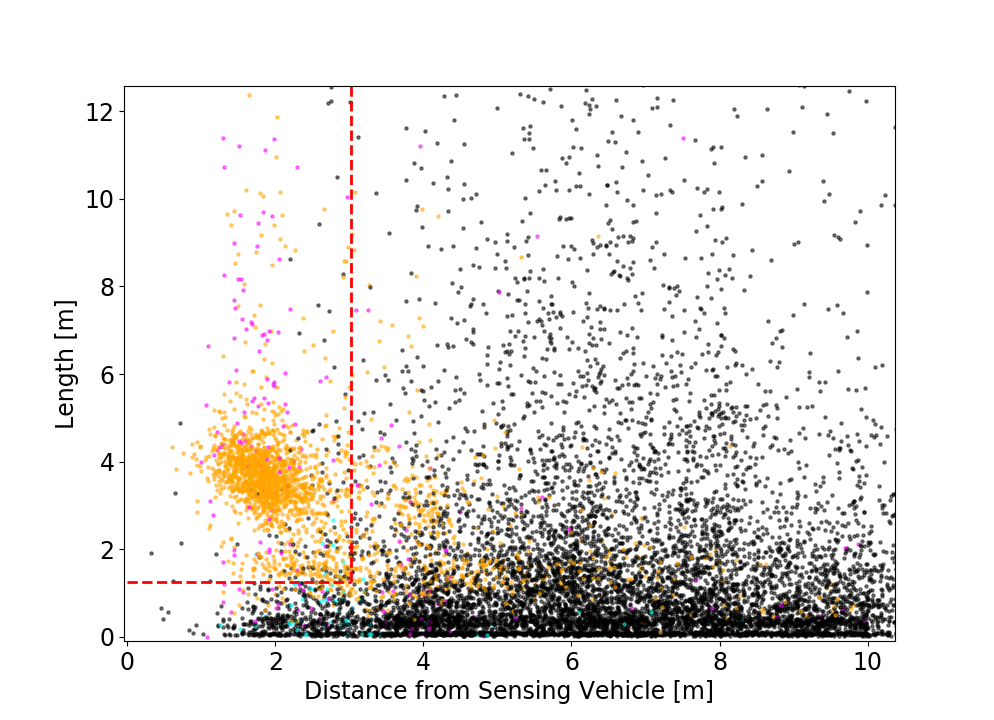
\includegraphics[width=\textwidth]{img/2d_length_distance_scatter_full_dataset_decision_tree_boundaries.png}
	\caption{A plot of the length and distance of the segments of the full dataset. Orange points show parking cars, while black points show free spaces. The red line shows the learned decision tree boundaries.}
	\label{fig:plot_2d_decision_tree}
\end{figure}

